\documentclass[11pt]{article}

\usepackage[margin=1in]{geometry}
\usepackage{amsmath,amssymb,amsthm}
\usepackage{graphicx}
\usepackage{hyperref}
\usepackage{listings}
\usepackage{xcolor}
\usepackage{booktabs}
\usepackage{tikz}
\usetikzlibrary{arrows.meta, positioning, shapes.geometric, fit, backgrounds}
\usepackage{microtype}
\usepackage{natbib}
\usepackage{authblk}
\usepackage{algorithm}
\usepackage{algpseudocode}

\hypersetup{
  colorlinks=true,
  linkcolor=blue!70!black,
  citecolor=blue!70!black,
  urlcolor=blue!70!black,
}

\lstset{
  basicstyle=\small\ttfamily,
  breaklines=true,
  frame=single,
  backgroundcolor=\color{gray!8},
  keywordstyle=\color{blue!70!black}\bfseries,
  commentstyle=\color{green!50!black},
  stringstyle=\color{red!70!black},
  numbers=left,
  numberstyle=\tiny\color{gray},
  numbersep=5pt,
}

\newtheorem{definition}{Definition}
\newtheorem{theorem}{Theorem}
\newtheorem{property}{Property}
\newtheorem{proposition}{Proposition}

\title{\textbf{Proof Protocol: A Verifiable Execution Layer\\
for AI-Generated and Programmatic Computation}}

\author[1]{Anonymous}
\affil[1]{Preprint — submitted to arXiv cs.CR / cs.DC}

\date{\today}

% ============================================================
\begin{document}
\maketitle

\begin{abstract}
We present \textsc{Proof Protocol}, a system that transforms arbitrary
computational claims — including those generated by large language models
(LLMs) — into verifiable, reproducible, and cryptographically signed
execution artifacts we call \emph{Computational Proof Objects} (CPOs).
A CPO binds a natural-language hypothesis, executable code, a controlled
sandbox specification, deterministic execution results, a SHA-256 content
hash, and an Ed25519 digital signature issued by the executing node.

Our core contribution is a \emph{replay-based verification model}: rather
than constructing zero-knowledge proofs, a verifier re-executes the same
code under identical constraints and compares observable outputs.  This
approach requires no trusted setup, no circuit compilation, and no global
consensus, while providing integrity, authenticity, and bounded
reproducibility under formally stated assumptions.  We define the CPO data
model, formalize the verification function as a decidable predicate,
characterize the cost structure of proof generation versus verification,
and analyze security properties with explicit non-goals.

The system supports seven isolated execution environments — \emph{worlds}
— spanning symbolic mathematics, probabilistic inference, evolutionary
computation, formal verification, and multimodal processing.  A reference
implementation in Python (FastAPI, Ed25519 via the \texttt{cryptography}
library, Docker) is publicly available.
\end{abstract}

\tableofcontents
\newpage

% ============================================================
\section{Introduction}
\label{sec:intro}

Modern AI systems and automated computation pipelines share a critical
weakness: their outputs are difficult to verify independently.  A language
model may produce a plausible-sounding numerical answer that is
arithmetically incorrect; a data-science pipeline may yield different
results on different machines; an autonomous agent may take actions whose
causal chain is impossible to reconstruct after the fact.

Three distinct communities experience this problem in parallel:

\paragraph{AI practitioners} observe that LLM outputs can \emph{hallucinate}
facts, including mathematical results, without any signal to the consumer
that the output is unreliable~\citep{ji2023survey}.  Grounding LLM outputs
in code execution partially addresses this, but does not provide an
auditable record.

\paragraph{Scientists} struggle with \emph{computational reproducibility}.
A 2016 survey found that more than 70\% of researchers had failed to
reproduce another scientist's results, with software environment differences
as a major contributing factor~\citep{baker2016reproducibility}.

\paragraph{Auditors and compliance engineers} require \emph{auditability}:
the ability to prove \emph{post hoc} that a particular output was produced
by a particular computation running in a particular environment.

Existing solutions address each concern in isolation.  Reproducibility
tools (MLflow~\citep{mlflow}, DVC~\citep{dvc}) log hyperparameters and
artifacts but do not cryptographically bind execution environments to
outputs.  Containerization (Docker, Nix~\citep{nix}) improves environment
reproducibility but does not attest to execution results.  Verifiable
computation systems (Truebit~\citep{truebit}, RISC Zero~\citep{risczero})
provide unconditional soundness via zero-knowledge proofs, but impose
circuit compilation overhead that is orders of magnitude larger than the
computation itself — making them impractical for lightweight interactive
use.

\textsc{Proof Protocol} occupies a different position in this design space:
a \emph{practical, lightweight verifiable execution layer} that
cryptographically binds computation inputs to outputs using replay-based
verification rather than zero-knowledge machinery.  The key insight is that
\emph{reproducible isolation is a sufficient substitute for cryptographic
universality} in many real-world settings: if the execution environment is
tightly controlled, re-execution is both cheap and conclusive.

\subsection*{Contributions}

\begin{enumerate}
  \item A formal data model for Computational Proof Objects (CPOs),
        including a definition of their content hash and node signature
        (Section~\ref{sec:model}).
  \item A formal, decidable verification function $\mathrm{Verify}$ with
        explicit assumptions and cost characterization
        (Sections~\ref{sec:verification},~\ref{sec:cost}).
  \item A formal definition of \emph{observable equivalence} that precisely
        specifies when two executions are considered equal
        (Section~\ref{sec:equivalence}).
  \item A security analysis with an explicit threat model and non-goals
        (Section~\ref{sec:security}).
  \item A reference implementation demonstrating practical deployability.
\end{enumerate}

% ============================================================
\section{The CPO Data Model}
\label{sec:model}

\begin{definition}[Computational Proof Object]
\label{def:cpo}
A \emph{Computational Proof Object} (CPO) is an immutable tuple
\[
  \mathcal{P} = (\textit{id},\; w,\; \textit{claim},\;
                  \textit{code},\; \textit{env},\; R,\; h,\; \sigma,\;
                  \textit{pk},\; t)
\]
where:
\begin{itemize}
  \item $\textit{id} \in \{0,1\}^{128}$ is a globally unique identifier
        (UUIDv4), sampled uniformly at proof-generation time.
  \item $w \in \mathcal{W}$ selects an execution environment from a finite,
        registered set of worlds (Section~\ref{sec:worlds}).
  \item $\textit{claim} \in \Sigma^*$ is a natural-language description of
        the hypothesis being tested.
  \item $\textit{code} \in \Sigma^*$ is the executable source code that
        operationalizes the claim.
  \item $\textit{env} = (\textit{image}, C)$ is an execution specification,
        where \textit{image} is an optional container image override and
        $C$ is a constraint map (memory limit, timeout, etc.).
  \item $R = (s_{\mathrm{out}},\, s_{\mathrm{err}},\, e,\, \tau)$ is the
        observed execution result: stdout, stderr, exit code, and wall-clock
        runtime in milliseconds.
  \item $h \in \{0,1\}^{256}$ is the content hash
        (Definition~\ref{def:hash}).
  \item $\sigma \in \{0,1\}^{512}$ is an Ed25519 signature over $h$
        produced by the node's private key $\mathit{sk}$.
  \item $\textit{pk} \in \{0,1\}^{256}$ is the Ed25519 public key of the
        signing node.
  \item $t \in \mathbb{Z}$ is the UTC Unix timestamp of creation.
\end{itemize}
\end{definition}

\begin{definition}[Content Hash]
\label{def:hash}
Let $\mathcal{P}^- = \mathcal{P} \setminus \{h, \sigma\}$ denote the CPO
with the mutable fields removed.  The content hash is:
\begin{equation}
  h(\mathcal{P}) \;=\; \mathrm{SHA\text{-}256}\bigl(
    \mathrm{canon}(\mathcal{P}^-)\bigr)
  \label{eq:hash}
\end{equation}
where $\mathrm{canon}$ is a deterministic serialization function
(Section~\ref{sec:canon}).
\end{definition}

The hash $h$ covers every semantically meaningful field, so tampering with
any single field produces a different hash that invalidates the stored
signature.

% ============================================================
\section{System Architecture}
\label{sec:architecture}

Figure~\ref{fig:architecture} illustrates the end-to-end pipeline.

\begin{figure}[h]
\centering
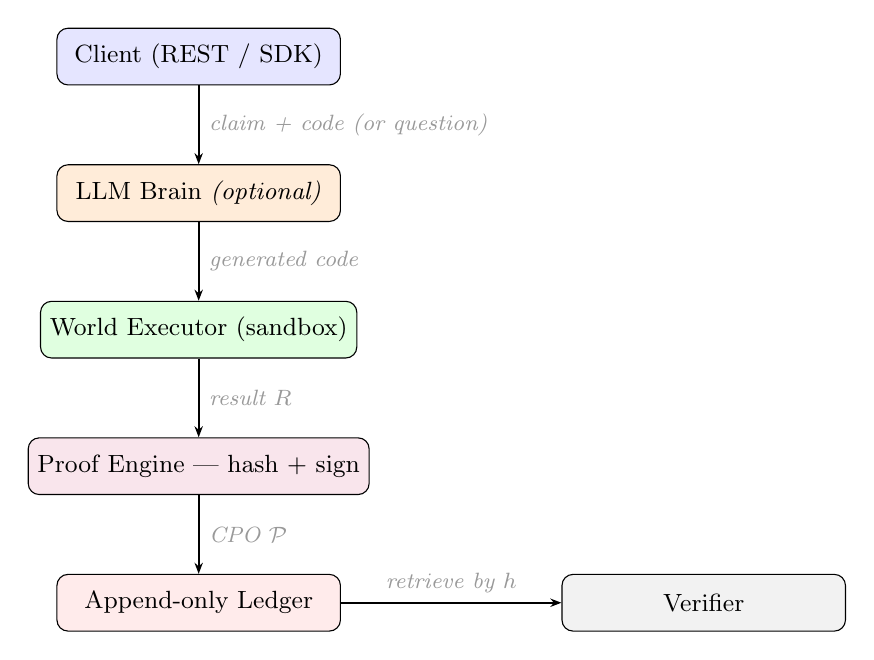
\begin{tikzpicture}[
  node distance=1.0cm and 1.2cm,
  box/.style={draw, rounded corners=4pt, minimum width=3.6cm,
              minimum height=0.72cm, align=center, font=\small},
  arrow/.style={-{Stealth[length=4pt]}, thick},
  lbl/.style={font=\footnotesize\itshape, text=gray!80},
]
\node[box, fill=blue!10]     (client) {Client (REST / SDK)};
\node[box, fill=orange!15,   below=of client]  (llm)    {LLM Brain \emph{(optional)}};
\node[box, fill=green!12,    below=of llm]     (exec)   {World Executor (sandbox)};
\node[box, fill=purple!10,   below=of exec]    (proof)  {Proof Engine — hash + sign};
\node[box, fill=red!8,       below=of proof]   (ledger) {Append-only Ledger};

\draw[arrow] (client) -- node[lbl,right]{claim + code (or question)} (llm);
\draw[arrow] (llm)    -- node[lbl,right]{generated \textit{code}}    (exec);
\draw[arrow] (exec)   -- node[lbl,right]{result $R$}                 (proof);
\draw[arrow] (proof)  -- node[lbl,right]{CPO $\mathcal{P}$}          (ledger);

\node[box, fill=gray!10, right=2.8cm of ledger] (verifier) {Verifier};
\draw[arrow] (ledger.east) -- node[lbl,above]{retrieve by $h$} (verifier.west);
\end{tikzpicture}
\caption{Proof Protocol pipeline.  The LLM brain is activated only by
\texttt{POST /ask}; direct code submission uses \texttt{POST /prove}.
Any stored CPO can be retrieved and re-verified offline via
\texttt{GET /verify/\{hash\}}.}
\label{fig:architecture}
\end{figure}

\paragraph{API surface.}  The system exposes four endpoints:

\begin{itemize}
  \item \texttt{POST /prove} — accept $(w, \textit{claim}, \textit{code})$,
        execute in sandbox, produce and store $\mathcal{P}$; return $h$ and
        $\sigma$.
  \item \texttt{POST /ask} — accept a natural-language question $q$,
        generate $\textit{code}$ via an LLM, then delegate to
        \texttt{/prove}.
  \item \texttt{GET /verify/\{h\}} — retrieve $\mathcal{P}$ by $h$,
        re-execute, return verification verdict.
  \item \texttt{GET /ledger} — browse the append-only log, optionally
        filtered by world $w$.
\end{itemize}

% ============================================================
\section{Execution Model}
\label{sec:execution}

\subsection{Bounded Execution Environment}

Each execution runs inside an ephemeral container with the following
constraints enforced at runtime:

\begin{itemize}
  \item \textbf{Network isolation}: all inbound and outbound traffic is
        suppressed (\texttt{network\_disabled=True}).
  \item \textbf{Read-only filesystem}: no persistent side effects
        (\texttt{read\_only=True}).
  \item \textbf{Memory cap}: default 128\,MiB; configurable via
        $\textit{env}.C$.
  \item \textbf{Execution timeout}: default $\delta = 10$\,s wall-clock.
  \item \textbf{Privilege suppression}: \texttt{no-new-privileges:true}
        blocks \texttt{setuid}-based escalation.
\end{itemize}

We call this combination a \emph{bounded execution environment} (BEE)
and denote the constraints as $\mathrm{BEE}(w, C)$.

\subsection{Observable Equivalence}
\label{sec:equivalence}

We define precisely when two execution results are considered equal during
verification.

\begin{definition}[Observable Equivalence]
\label{def:equiv}
Let $R = (s_{\mathrm{out}}, s_{\mathrm{err}}, e, \tau)$ and
$R' = (s'_{\mathrm{out}}, s'_{\mathrm{err}}, e', \tau')$ be two execution
results.  We say $R \approx R'$ (\emph{observably equivalent}) if and only
if:
\begin{align}
  \mathrm{norm}(s_{\mathrm{out}}) &= \mathrm{norm}(s'_{\mathrm{out}}) \label{eq:stdout} \\
  e &= e' \label{eq:exit}
\end{align}
where $\mathrm{norm}(s) = s.\mathrm{strip}()$ removes leading and trailing
whitespace and normalizes line endings to \texttt{\textbackslash n}.
\end{definition}

The stderr stream and runtime $\tau$ are deliberately excluded from
$\approx$: stderr content can vary with library version, and runtime is
non-deterministic by nature.  Only the semantic output (stdout) and success
indicator (exit code) are equality-tested.

\begin{definition}[Bounded Determinism]
\label{def:det}
A code/environment pair $(\textit{code}, \mathrm{BEE}(w, C))$ is
\emph{boundedly deterministic} if for all executions $E_1, E_2$ producing
results $R_1, R_2$:
\[
  R_1 \approx R_2
\]
\end{definition}

Bounded determinism is a \emph{sufficient}, not necessary, condition for
successful re-verification.  Stochastic programs can still be verified for
integrity and authenticity (steps 1--2 of Algorithm~\ref{alg:verify}) even
when output equality (steps 3--4) does not hold.

% ============================================================
\section{Cryptographic Layer}
\label{sec:crypto}

\subsection{Canonical Serialization}
\label{sec:canon}

To ensure $h$ is stable across serialization implementations, we compute
$\mathrm{canon}$ using an RFC~8785-inspired deterministic JSON form: keys
are sorted lexicographically at every nesting level, separators carry no
extra whitespace, and Unicode code points are preserved without escaping:
\[
  \mathrm{canon}(O) \;=\;
    \texttt{JSON.dumps}\!\left(O,\;
    \texttt{sort\_keys=True},\;
    \texttt{separators=(",",":")},\;
    \texttt{ensure\_ascii=False}\right)
\]
This ensures that two identical CPOs serialized independently produce
bitwise-identical byte strings before hashing.

\subsection{Content Hash and Signature}

The content hash (Equation~\eqref{eq:hash}) is computed over the UTF-8
encoding of $\mathrm{canon}(\mathcal{P}^-)$.  The node signs the
hex-encoded hash string:
\[
  \sigma \;=\; \mathrm{Ed25519.Sign}(\mathit{sk},\;
    \mathrm{hex}(h) \cdot \text{UTF-8})
\]

\begin{property}[Tamper Evidence]
\label{prop:tamper}
For any CPO $\mathcal{P}$ and any field $f \in \mathcal{P}^-$, the
modified tuple $\mathcal{P}[f \mapsto f']$ satisfies
$h(\mathcal{P}[f \mapsto f']) \neq h(\mathcal{P})$ with probability
$1 - 2^{-256}$ (SHA-256 collision resistance), which implies
$\mathrm{Ed25519.Verify}(\mathit{pk},\, h',\, \sigma) = \bot$.
\end{property}

\subsection{Node Identity}

Each node generates an Ed25519 keypair at first startup.  The node
identifier is a human-readable prefix:
\[
  \textit{node\_id} \;=\;
    \mathrm{hex}(\mathrm{SHA\text{-}256}(\mathit{pk}))[\,{:}16\,]
\]
The full public key $\mathit{pk}$ is stored inline in every CPO, so
verification requires no external key registry.

% ============================================================
\section{World Abstraction}
\label{sec:worlds}

A \emph{world} $w \in \mathcal{W}$ is a named, versioned OCI container
image providing a specific runtime with its library ecosystem and
behavioral assumptions.

\begin{table}[h]
\centering
\caption{Registered worlds ($|\mathcal{W}| = 7$) and their runtime environments.
Worlds marked \emph{bounded} are stochastic by design; re-verification
confirms integrity but not output equality without explicit seed fixation.}
\label{tab:worlds}
\begin{tabular}{lllc}
\toprule
\textbf{World} & \textbf{Primary domain} & \textbf{Key libraries}
  & \textbf{Output equality} \\
\midrule
\texttt{llm}          & General Python           & stdlib               & exact \\
\texttt{symbolic}     & Symbolic mathematics     & SymPy, Z3            & exact \\
\texttt{formal}       & Logic / SMT solving      & Z3, py-aiger         & exact \\
\texttt{bayesian}     & Probabilistic inference  & NumPyro, PyMC        & bounded \\
\texttt{evolutionary} & Agent-based simulation   & DEAP, Mesa           & bounded \\
\texttt{multimodal}   & Vision / audio           & PyTorch CPU, Pillow  & exact \\
\texttt{neuro}        & Neural pipeline tooling  & DSPy, LangChain      & bounded \\
\bottomrule
\end{tabular}
\end{table}

% ============================================================
\section{Verification Procedure}
\label{sec:verification}

\subsection{Formal Verification Function}

\begin{definition}[Verification Predicate]
\label{def:verify}
Let $\mathcal{P}$ be a CPO retrieved from the ledger by content hash $h$.
Define the boolean verification predicate:
\begin{equation}
  \mathrm{Verify}(\mathcal{P}) \;=\;
    \underbrace{\mathrm{SigOK}(\mathcal{P})}_{\text{authenticity}}
    \;\land\;
    \underbrace{\mathrm{HashOK}(\mathcal{P})}_{\text{integrity}}
    \;\land\;
    \underbrace{\mathrm{ReplayOK}(\mathcal{P})}_{\text{reproducibility}}
  \label{eq:verify}
\end{equation}
where:
\begin{align}
  \mathrm{SigOK}(\mathcal{P})   &\;\triangleq\;
    \mathrm{Ed25519.Verify}(\mathcal{P}.\mathit{pk},\;
                             \mathcal{P}.h,\;
                             \mathcal{P}.\sigma) \label{eq:sigok} \\[4pt]
  \mathrm{HashOK}(\mathcal{P})  &\;\triangleq\;
    h(\mathcal{P}) \;=\; \mathcal{P}.h \label{eq:hashok} \\[4pt]
  \mathrm{ReplayOK}(\mathcal{P}) &\;\triangleq\;
    \mathrm{Exec}(\mathcal{P}.\textit{code},\;
                   \mathrm{BEE}(\mathcal{P}.w,\; \mathcal{P}.\textit{env}.C))
    \;\approx\;
    \mathcal{P}.R \label{eq:replayok}
\end{align}
and $\mathrm{Exec}$ denotes a fresh sandbox execution returning result
$R'$.
\end{definition}

The three sub-predicates are independent and provide layered guarantees:
$\mathrm{SigOK}$ and $\mathrm{HashOK}$ require only the stored CPO (no
re-execution); $\mathrm{ReplayOK}$ requires re-execution and holds only
under bounded determinism (Definition~\ref{def:det}).

\subsection{Algorithm}

Algorithm~\ref{alg:verify} gives the procedural form used in the
implementation.  Figure~\ref{fig:verify-flow} visualizes the decision flow.

\begin{algorithm}[h]
\caption{$\mathrm{Verify}(\mathcal{P})$}
\label{alg:verify}
\begin{algorithmic}[1]
\Require CPO $\mathcal{P}$ retrieved from ledger by $h$
\Ensure Boolean verdict $v \in \{\top, \bot\}$, reason string
\State $h' \gets \mathrm{SHA\text{-}256}(\mathrm{canon}(\mathcal{P}^-))$
\If{$h' \neq \mathcal{P}.h$}
  \Return $(\bot,\; \text{"hash mismatch"})$
\EndIf
\If{$\neg\,\mathrm{Ed25519.Verify}(\mathcal{P}.\mathit{pk},\; h',\; \mathcal{P}.\sigma)$}
  \Return $(\bot,\; \text{"invalid signature"})$
\EndIf
\State $R' \gets \mathrm{Exec}(\mathcal{P}.\textit{code},\;
                                \mathrm{BEE}(\mathcal{P}.w,\; \mathcal{P}.\textit{env}.C))$
\If{$\mathrm{norm}(R'.\textit{stdout}) \neq \mathrm{norm}(\mathcal{P}.R.\textit{stdout})$}
  \Return $(\bot,\; \text{"stdout mismatch"})$
\EndIf
\If{$R'.\textit{exit\_code} \neq \mathcal{P}.R.\textit{exit\_code}$}
  \Return $(\bot,\; \text{"exit code mismatch"})$
\EndIf
\Return $(\top,\; \text{"verified"})$
\end{algorithmic}
\end{algorithm}

\begin{figure}[h]
\centering
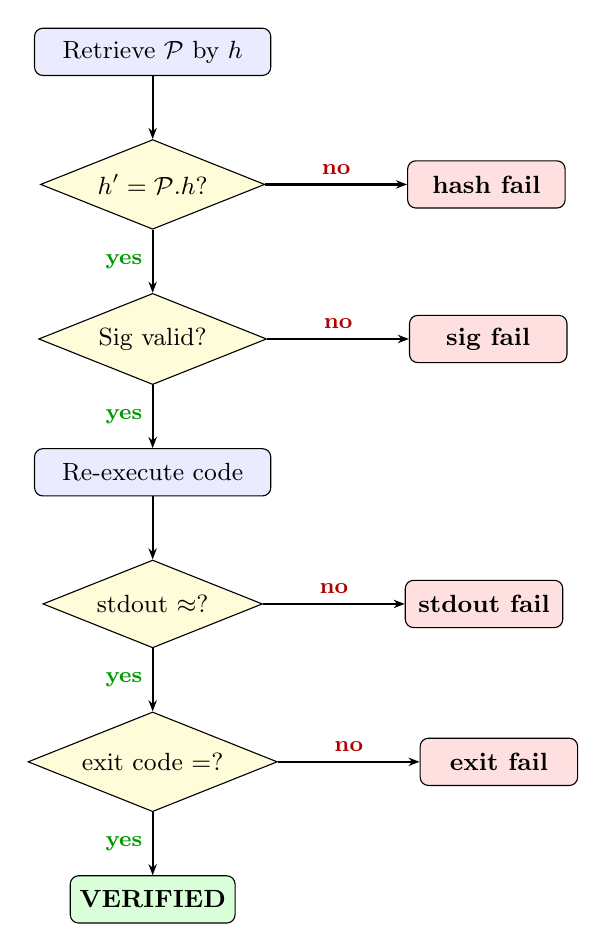
\begin{tikzpicture}[
  node distance=0.8cm and 1.5cm,
  decision/.style={diamond, draw, fill=yellow!15, aspect=2.5,
                   minimum height=0.7cm, align=center, font=\small},
  process/.style={draw, rounded corners=3pt, fill=blue!8,
                  minimum width=3cm, minimum height=0.6cm,
                  align=center, font=\small},
  result/.style={draw, rounded corners=3pt, minimum width=2cm,
                 minimum height=0.6cm, align=center, font=\small\bfseries},
  arrow/.style={-{Stealth[length=4pt]}, thick},
  yes/.style={font=\footnotesize\color{green!60!black}},
  no/.style={font=\footnotesize\color{red!70!black}},
]
\node[process]   (start)  {Retrieve $\mathcal{P}$ by $h$};
\node[decision,  below=of start]  (d1) {$h' = \mathcal{P}.h$?};
\node[decision,  below=of d1]     (d2) {Sig valid?};
\node[process,   below=of d2]     (exec) {Re-execute code};
\node[decision,  below=of exec]   (d3) {stdout $\approx$?};
\node[decision,  below=of d3]     (d4) {exit code $=$?};
\node[result,    below=of d4, fill=green!15] (ok)   {VERIFIED};
\node[result,    right=1.8cm of d1, fill=red!12] (f1)  {hash fail};
\node[result,    right=1.8cm of d2, fill=red!12] (f2)  {sig fail};
\node[result,    right=1.8cm of d3, fill=red!12] (f3)  {stdout fail};
\node[result,    right=1.8cm of d4, fill=red!12] (f4)  {exit fail};

\draw[arrow] (start) -- (d1);
\draw[arrow] (d1) -- node[yes,left]{\textbf{yes}} (d2);
\draw[arrow] (d1) -- node[no,above]{\textbf{no}} (f1);
\draw[arrow] (d2) -- node[yes,left]{\textbf{yes}} (exec);
\draw[arrow] (d2) -- node[no,above]{\textbf{no}} (f2);
\draw[arrow] (exec) -- (d3);
\draw[arrow] (d3) -- node[yes,left]{\textbf{yes}} (d4);
\draw[arrow] (d3) -- node[no,above]{\textbf{no}} (f3);
\draw[arrow] (d4) -- node[yes,left]{\textbf{yes}} (ok);
\draw[arrow] (d4) -- node[no,above]{\textbf{no}} (f4);
\end{tikzpicture}
\caption{Decision flow of $\mathrm{Verify}$ (Algorithm~\ref{alg:verify}).
Steps 1--2 test integrity and authenticity without re-execution.
Steps 3--4 test reproducibility and require a fresh sandbox run.}
\label{fig:verify-flow}
\end{figure}

\begin{proposition}[Verify is Decidable]
Algorithm~\ref{alg:verify} terminates in finite time for any input
$\mathcal{P}$, because: (i) $\mathrm{SHA\text{-}256}$ and
$\mathrm{Ed25519.Verify}$ run in $O(|\mathrm{canon}(\mathcal{P}^-)|)$ time;
(ii) $\mathrm{Exec}$ is bounded by the timeout $\delta \in \mathcal{P}.\textit{env}.C$;
(iii) $\mathrm{norm}$ and equality checks are $O(|s_{\mathrm{out}}|)$.
\end{proposition}

% ============================================================
\section{Cost Analysis}
\label{sec:cost}

A key advantage of replay-based verification over ZK-based systems is its
\emph{symmetric cost structure}: verification costs approximately the same
as proof generation, rather than imposing a proving overhead.

\subsection{Proof Generation}

Let $T_{\mathrm{exec}}$ be the sandbox execution time for code of input
size $n$.  Proof generation incurs:

\begin{enumerate}
  \item \textbf{Sandbox execution}: $T_{\mathrm{exec}}(n)$ — the dominant term.
  \item \textbf{Canonical serialization}: $O(|\mathcal{P}|)$ — proportional
        to CPO size, typically $O(n + |s_{\mathrm{out}}|)$.
  \item \textbf{SHA-256 hash}: $O(|\mathrm{canon}(\mathcal{P}^-)|)$ —
        hardware-accelerated on modern CPUs; negligible in practice.
  \item \textbf{Ed25519 sign}: $O(1)$ — constant time, $\approx 50\,\mu$s
        on commodity hardware.
\end{enumerate}

Total: $T_{\mathrm{prove}} = T_{\mathrm{exec}}(n) + O(|\mathcal{P}|)$.

\subsection{Verification}

Verification adds one re-execution to steps (2)--(4) above:
\[
  T_{\mathrm{verify}} = T'_{\mathrm{exec}}(n) + O(|\mathcal{P}|)
                       + O(|s_{\mathrm{out}}|)
\]
where $T'_{\mathrm{exec}}$ is the re-execution time.  Under bounded
determinism, $T'_{\mathrm{exec}} \approx T_{\mathrm{exec}}$.  The
cryptographic overhead is $O(|\mathcal{P}|)$ and empirically sub-millisecond.

\subsection{Comparison with ZK-based Systems}

In ZK-based systems (e.g., RISC Zero), proving time is
$T_{\mathrm{ZK}} \approx \alpha \cdot T_{\mathrm{exec}}$ where
$\alpha \gg 1$ (commonly $10^3$--$10^6\times$ depending on circuit complexity),
and verification is $O(|proof|)$ — much cheaper.
\textsc{Proof Protocol} reverses this asymmetry:

\begin{table}[h]
\centering
\caption{Cost structure comparison.}
\label{tab:cost}
\begin{tabular}{lll}
\toprule
\textbf{System} & \textbf{Proof generation} & \textbf{Verification} \\
\midrule
\textsc{Proof Protocol} & $T_{\mathrm{exec}} + O(|\mathcal{P}|)$
                         & $T_{\mathrm{exec}} + O(|\mathcal{P}|)$ \\
ZK (e.g., RISC Zero)    & $\alpha \cdot T_{\mathrm{exec}},\; \alpha \gg 1$
                         & $O(|\textit{proof}|)$                    \\
\bottomrule
\end{tabular}
\end{table}

Replay-based verification is preferable when re-execution is cheap, the
verifier controls or trusts the execution environment, and ZK overhead is
prohibitive.  ZK systems are preferable when re-execution is impossible or
the verifier has no access to a trusted runtime.

% ============================================================
\section{Security Analysis}
\label{sec:security}

\subsection{Threat Model}

We analyze three adversary classes:

\paragraph{Passive ledger reader.}
An adversary who reads CPOs from the ledger but cannot modify them.  The
append-only storage structure and Property~\ref{prop:tamper} ensure that any
modification is detectable.

\paragraph{Malicious code submitter.}
An adversary who submits code intended to escape the sandbox or cause
persistent side effects on the host.  The BEE constraints (network
isolation, read-only FS, memory cap, no-new-privileges) collectively reduce
the surface area.  We note that Docker-based isolation does not defend
against kernel-level exploits (see Section~\ref{sec:limitations}).

\paragraph{Compromised node.}
An adversary who controls a node's private key $\mathit{sk}$.  This
adversary can forge signatures for any claim, but every CPO carries
$\mathit{pk}$ inline, so attribution is possible.  Key rotation invalidates
future attestations; past CPOs remain verifiable against the original
$\mathit{pk}$.

\subsection{Non-Goals}

\textsc{Proof Protocol} explicitly does not provide:

\begin{itemize}
  \item \textbf{Semantic correctness}: $\mathrm{Verify}(\mathcal{P}) = \top$
        proves that \textit{code} ran and produced \textit{stdout}.  It does
        not prove that \textit{stdout} correctly answers \textit{claim}.
  \item \textbf{Universal soundness}: unlike ZK proofs, a successful replay
        depends on environmental determinism, which is assumed not proved.
  \item \textbf{Global consensus}: no mechanism prevents two nodes from
        issuing conflicting CPOs for the same claim.
  \item \textbf{Confidentiality}: CPOs store \textit{code} and
        \textit{stdout} in plaintext.
  \item \textbf{Kernel isolation}: Docker shares the host kernel.
\end{itemize}

% ============================================================
\section{Limitations}
\label{sec:limitations}

\paragraph{Determinism scope.}
Stochastic worlds (Bayesian, Evolutionary, Neuro) cannot guarantee
$R \approx R'$ without explicit random seed fixation in the submitted code.
Submitters should set seeds to obtain full $\mathrm{Verify} = \top$;
otherwise, only $\mathrm{SigOK} \land \mathrm{HashOK}$ is guaranteed.

\paragraph{Container security boundary.}
Docker-based isolation does not protect against kernel exploits.  A hardened
deployment should use microVM isolation (Firecracker~\citep{firecracker}) or
a syscall-intercepting runtime (gVisor~\citep{gvisor}).

\paragraph{LLM code quality.}
The \texttt{/ask} endpoint relies on an LLM to generate \emph{correct} code.
A hallucinated or buggy code snippet produces a valid, signed CPO for a
wrong answer: $\mathrm{Verify} = \top$ with incorrect semantics.  Users
should treat CPOs as execution certificates, not semantic truth certificates.

\paragraph{Ledger scalability.}
The current JSONL ledger is append-only and single-file.  At scale,
partitioning by world or time window, or migration to a structured event
store (Kafka, RocksDB), is required.

\paragraph{Single-node trust.}
Each node is independently trusted.  Quorum-based cross-node verification
(requiring $k$-of-$n$ agreeing nodes) is a planned extension.

% ============================================================
\section{Related Work}
\label{sec:related}

\paragraph{Reproducible research and ML tracking.}
MLflow~\citep{mlflow} and DVC~\citep{dvc} record experiment parameters and
artifacts but do not cryptographically bind execution environments to
outputs.  Nix~\citep{nix} and Guix provide reproducible builds at the
software delivery level, not at the runtime execution level.

\paragraph{Verifiable computation.}
Truebit~\citep{truebit} introduces interactive dispute resolution for
on-chain verification of off-chain computation.  RISC Zero~\citep{risczero}
and StarkWare compile arbitrary programs to ZK circuits, providing
computational soundness at the cost of $10^3$--$10^6\times$ proving
overhead.  Cartesi~\citep{cartesi} runs Linux in a reproducible RISC-V
machine, generating verifiable traces.  \textsc{Proof Protocol} trades
unconditional soundness for practical deployability: re-execution is
sufficient when the verifier controls or trusts the runtime.

\paragraph{Trusted Execution Environments.}
Intel SGX and AMD SEV provide hardware attestation of code running in
enclaves~\citep{sgx}, offering strong isolation without network trust
assumptions.  These require specific hardware and attestation
infrastructure; \textsc{Proof Protocol} is hardware-agnostic.

\paragraph{Secure sandboxing.}
Firecracker~\citep{firecracker} provides microVM isolation with
sub-125\,ms boot times, used in AWS Lambda.  gVisor~\citep{gvisor}
intercepts syscalls in user space.  Both are compatible with our execution
layer and represent a natural isolation upgrade path.

\paragraph{LLM grounding via tool use.}
Toolformer~\citep{toolformer} and ReAct~\citep{react} ground LLM outputs
in external tool calls to reduce hallucination.  The \texttt{/ask}
endpoint instantiates this paradigm with a verifiable execution backend:
the LLM proposes code, the sandbox executes it, and the CPO attests to the
result.

\paragraph{Execution provenance.}
PROV-DM~\citep{provdm} and related W3C provenance standards model
provenance graphs for data pipelines.  \textsc{Proof Protocol} can be
viewed as a lightweight cryptographic specialization of execution provenance
for sandboxed programs.

% ============================================================
\section{Conclusion}
\label{sec:conclusion}

We have presented \textsc{Proof Protocol}, a lightweight verifiable
execution layer that transforms computational claims into signed, auditable,
and reproducible artifacts.  The system rests on three principles:

\begin{enumerate}
  \item \textbf{Isolation implies reproducibility.}  A bounded execution
        environment makes replay-based verification tractable without ZK
        machinery.
  \item \textbf{Canonical hashing implies integrity.}  Any tamper with a
        CPO is detectable by recomputing $h$ (Property~\ref{prop:tamper}).
  \item \textbf{Signed attestation implies non-repudiation.}  Node identity
        is cryptographically bound to every CPO it issues.
\end{enumerate}

We formalized the CPO data model, defined observable equivalence precisely
(Definition~\ref{def:equiv}), expressed the verification function as a
decidable predicate (Definition~\ref{def:verify} and
Algorithm~\ref{alg:verify}), and characterized the symmetric cost structure
that distinguishes replay-based from ZK-based verification.  These
properties jointly position \textsc{Proof Protocol} as a practical trust
layer for AI pipelines, scientific computation, autonomous agents, and
auditable decision systems.

\paragraph{Availability.}
The reference implementation (Python, FastAPI, Ed25519, Docker) is
available at \url{https://github.com/haynbroit-alt/CPO}.

% ============================================================
\bibliographystyle{plainnat}
\begin{thebibliography}{99}

\bibitem[Baker(2016)]{baker2016reproducibility}
Baker, M. (2016).
\newblock 1,500 scientists lift the lid on reproducibility.
\newblock \emph{Nature}, 533(7604):452--454.

\bibitem[Machado et al.(2021)]{cartesi}
Machado, D., et al. (2021).
\newblock Cartesi: Bringing real-world computations to the blockchain.
\newblock \emph{arXiv preprint arXiv:2109.04316}.

\bibitem[Agache et al.(2020)]{firecracker}
Agache, A., et al. (2020).
\newblock Firecracker: Lightweight virtualization for serverless applications.
\newblock In \emph{17th USENIX NSDI}, pp.\ 419--434.

\bibitem[Costan \& Devadas(2016)]{sgx}
Costan, V., and Devadas, S. (2016).
\newblock Intel SGX explained.
\newblock \emph{IACR ePrint Archive}, 2016:086.

\bibitem[Ji et al.(2023)]{ji2023survey}
Ji, Z., et al. (2023).
\newblock Survey of hallucination in natural language generation.
\newblock \emph{ACM Computing Surveys}, 55(12):1--38.

\bibitem[Zaharia et al.(2018)]{mlflow}
Zaharia, M., et al. (2018).
\newblock Accelerating the machine learning lifecycle with MLflow.
\newblock \emph{IEEE Data Engineering Bulletin}, 41(4):39--45.

\bibitem[Rumelhart et al.(2020)]{dvc}
Ruslan, K., et al. (2020).
\newblock DVC: Data version control — git for data and models.
\newblock \url{https://dvc.org}.

\bibitem[Dolstra(2006)]{nix}
Dolstra, E. (2006).
\newblock \emph{The Purely Functional Software Deployment Model}.
\newblock PhD thesis, Utrecht University.

\bibitem[Lacasse et al.(2020)]{gvisor}
Lacasse, N., et al. (2020).
\newblock gVisor: An application kernel for containers.
\newblock \emph{USENIX HotCloud}.

\bibitem[Teutsch \& Reitwie{\ss}ner(2019)]{truebit}
Teutsch, J., and Reitwie{\ss}ner, C. (2019).
\newblock A scalable verification solution for blockchains.
\newblock \emph{arXiv preprint arXiv:1908.04756}.

\bibitem[Schick et al.(2023)]{toolformer}
Schick, T., et al. (2023).
\newblock Toolformer: Language models can teach themselves to use tools.
\newblock In \emph{Advances in NeurIPS 36}.

\bibitem[Yao et al.(2023)]{react}
Yao, S., et al. (2023).
\newblock ReAct: Synergizing reasoning and acting in language models.
\newblock In \emph{ICLR 2023}.

\bibitem[RISC Zero(2022)]{risczero}
RISC Zero. (2022).
\newblock RISC Zero: A general-purpose zero-knowledge virtual machine.
\newblock \url{https://www.risczero.com}.

\bibitem[Lebo et al.(2013)]{provdm}
Lebo, T., et al. (2013).
\newblock PROV-DM: The PROV Data Model.
\newblock W3C Recommendation. \url{https://www.w3.org/TR/prov-dm/}.

\end{thebibliography}

\end{document}
